\documentclass{book}

\usepackage{fontspec} % used to import Calibri
\usepackage{anyfontsize} % used to adjust font size

% needed for inch and other length measurements
% to be recognized
\usepackage{calc}

% for colors and text effects as is hopefully obvious
\usepackage[dvipsnames]{xcolor}
\usepackage{soul}

% control over margins
\usepackage[margin=1in]{geometry}
\usepackage[strict]{changepage}

\usepackage{mathtools}
\usepackage{amsfonts}
\usepackage{bm}

\usepackage[scr=rsfso, scrscaled=.96]{mathalpha}

% This is how I'm getting the nice caligraphy font :(
\DeclareMathAlphabet{\eulerscr}{U}{eus}{m}{n}
\newcommand{\mathcalli}[1]{\text{\scalebox{1.11}{$\eulerscr{#1}$}}}


\usepackage{amssymb} % originally imported to get the proof square
\usepackage{xfrac}
\usepackage[overcommands]{overarrows} % Get my preferred vector arrows...
\usepackage{relsize}

% Just am using this to get a dashed line in a table...
% Also you apparently want this to be inactive if you aren't
% using it because it slows compilation.
\usepackage{arydshln} \ADLinactivate 
\newenvironment{allowTableDashes}{\ADLactivate}{\ADLinactivate}

\usepackage{graphicx}
\graphicspath{{./158_Images/}}

\usepackage{tikz}
   \usetikzlibrary{arrows.meta}
   \usetikzlibrary{graphs, graphs.standard}

\usepackage{quiver} %commutative diagrams






\usepackage[hidelinks]{hyperref}
\newcommand{\inLinkRap}[2]{{\color{blue}\hyperlink{#1}{\textit{#2}}}}







\newfontfamily{\calibri}{Calibri}
\setlength{\parindent}{0pt}
\definecolor{RawerSienna}{HTML}{945D27}

% ~~~~~~~~~~~~~~~~~~~~~~~~~~~~~~~~~~~~~~~~~~~~~~~~~~
%Arrow Commands:

% Thank you Bernard, gernot, and Sigur who I copied this from:
% https://tex.stackexchange.com/questions/364096/command-for-longhookrightarrow
\renewcommand{\hookrightarrow}{\lhook\joinrel\rightarrow}
\renewcommand{\hookleftarrow}{\leftarrow\joinrel\rhook}
\newcommand{\hooklongrightarrow}{\lhook\joinrel\longrightarrow}
\newcommand{\hooklongleftarrow}{\longleftarrow\joinrel\rhook}
\newcommand{\hookxlongrightarrow}[2][]{\lhook\joinrel\xrightarrow[#1]{#2}}
\newcommand{\hookxlongleftarrow}[2][]{\xleftarrow[#1]{#2}\joinrel\rhook}

% Thank you egreg who I copied from:
% https://tex.stackexchange.com/questions/260554/two-headed-version-of-xrightarrow
\newcommand{\longrightarrowdbl}{\longrightarrow\mathrel{\mkern-14mu}\rightarrow}
\newcommand{\longleftarrowdbl}{\leftarrow\mathrel{\mkern-14mu}\longleftarrow}

\newcommand{\xrightarrowdbl}[2][]{%
  \xrightarrow[#1]{#2}\mathrel{\mkern-14mu}\rightarrow
}
\newcommand{\xleftarrowdbl}[2][]{%
  \leftarrow\mathrel{\mkern-14mu}\xleftarrow[#1]{#2}
}

\newcommand{\mRoman}[1]{%
   \textrm{\MakeUppercase{\romannumeral #1}}%
}



% ~~~~~~~~~~~~~~~~~~~~~~~~~~~~~~~~~~~~~~~~~~~~~~~~~~

\newcommand{\hOne}{%
   \color{Black}%
   \fontsize{14}{16}\selectfont%
}
\newcommand{\hTwo}{%
\color{Black}%
   \fontsize{13}{15}\selectfont%
}
% \newcommand{\scratchWork}{%
%    \color{PineGreen!85!Orange}
%    \fontsize{12}{14}\selectfont%
% }
\newcommand{\hThree}{%
   \color{Black}%
   \fontsize{12}{14}\selectfont%
}
\newcommand{\myComment}{%
   \color{RawerSienna}%
   \fontsize{12}{14}\selectfont%
}
\newcommand{\pracOne}{
   \color{BrickRed}%
   \fontsize{13}{15}\selectfont%
}
\newcommand{\pracTwo}{
   \color{Orange}%
   \fontsize{12}{14}\selectfont%
}
\newcommand{\why}{%
   \color{Orange}%
   \fontsize{12}{14}\selectfont%
	Why:
}
\newcommand{\exOne}{%
   \color{Purple}%
   \fontsize{14}{16}\selectfont%
}
\newcommand{\exTwo}{%
   \color{Purple}%
   \fontsize{13}{15}\selectfont%
}
\newcommand{\exThree}{%
   \color{Purple}%
   \fontsize{12}{14}\selectfont%
}
\newcommand{\exP}{%
   \color{Purple}%
   \fontsize{12}{14}\selectfont%
}
\newcommand{\exTwoP}{%
   \color{RedViolet}%
   \fontsize{13}{15}\selectfont%
}
\newcommand{\exThreeP}{%
   \color{RedViolet}%
   \fontsize{12}{14}\selectfont%
}
\newcommand{\exFourP}{%
   \color{RedViolet}%
   \fontsize{11}{13}\selectfont%
}
\newcommand{\exPP}{%
   \color{RedViolet}%
   \fontsize{12}{14}\selectfont%
}
\newcommand{\exPPP}{%
   \color{VioletRed}%
   \fontsize{12}{14}\selectfont%
}

% Homework standard below (God the bloat in the header is absurd...)
% ~~~~~~~~~~~~~~~~~~~~~~~~~~~~~~~~~~~~~~~~~~~~~~~~
\newcommand{\Hstatement}{%
   \color{MidnightBlue!90!Black}%
   \fontsize{12}{13}\selectfont%
}
\newcommand{\HexOne}{%
   \color{Purple}%
   \fontsize{12}{13}\selectfont%
}
\newcommand{\HexTwoP}{%
   \color{RedViolet}%
   \fontsize{12}{13}\selectfont%
}
\newcommand{\HexPPP}{%
   \color{VioletRed}%
   \fontsize{11}{12}\selectfont%
}

% ~~~~~~~~~~~~~~~~~~~~~~~~~~~~~~~~~~~~~~~~~~~~~~~~

\newcommand{\cyPen}[1]{{\vphantom{.}\color{Cerulean}#1}}
\newcommand{\redPen}[1]{{\vphantom{.}\color{Red}#1}}

\newenvironment{myIndent}{%
   \begin{adjustwidth}{2.5em}{0em}%
}{%
   \end{adjustwidth}%
}

\newenvironment{myDindent}{%
   \begin{adjustwidth}{5em}{0em}%
}{%
   \end{adjustwidth}%
}

\newenvironment{myTindent}{%
   \begin{adjustwidth}{7.5em}{0em}%
}{%
   \end{adjustwidth}%
}

\newenvironment{myConstrict}{%
   \begin{adjustwidth}{2.5em}{2.5em}%
}{%
   \end{adjustwidth}%
}

\newcommand{\udefine}[1]{{%
   \setulcolor{Red}%
   \setul{0.14em}{0.07em}%
   \ul{#1}%
}}

\newcommand{\uprop}[1]{{%
   \setulcolor{Purple}%
   \setul{0.14em}{0.07em}%
   \ul{#1} 
}}

\newcommand{\blab}[1]{\textbf{#1}}
\newcommand{\blect}[1]{{\color{MidnightBlue}\textbf{#1}}}

\newcommand{\uuline}[2][.]{%
{\vphantom{a}\color{#1}%
\rlap{\rule[-0.18em]{\widthof{#2}}{0.06em}}%
\rlap{\rule[-0.32em]{\widthof{#2}}{0.06em}}}%
#2}

\newcommand{\pprime}{{\prime\prime}}
\newcommand{\suchthat}{ \hspace{0.3em}s.t.\hspace{0.3em}}
\newcommand{\rea}[1]{\mathrm{Re}(#1)}
\newcommand{\ima}[1]{\mathrm{Im}(#1)}
\newcommand{\comp}{\mathsf{C}}
\newcommand{\trans}{\mathsf{T}}
\newcommand{\myHS}{ \hspace{0.5em}}
\newcommand{\gap}{\phantom{2}}

\newcommand{\GenLin}{\ensuremath{\mathrm{GL}}}
\newcommand{\Cay}{\ensuremath{\mathrm{Cay}}}

\newcommand{\myId}{\mathrm{Id}}
\newcommand{\myIm}{\mathrm{im}}
\newcommand{\Obj}{\mathrm{Obj}}
\newcommand{\Hom}{\mathrm{Hom}}
\newcommand{\End}{\mathrm{End}}
\newcommand{\Aut}{\mathrm{Aut}}

\newcommand{\df}{\mathrm{d}}
\newcommand{\Df}{\mathrm{D}}

\newcommand{\mcateg}[1]{{\bm{\mathsf{#1}}}}

\newcommand{\mdeg}{\mathrm{mdeg}\phantom{.}}

\newcommand{\divides}{\mathop{\mid}}

\newcommand{\card}{\mathrm{card}}
\newcommand{\supp}{\mathrm{supp}}
\newcommand{\diam}{\mathrm{diam}}
\newcommand{\conv}{\mathrm{conv}}
\newcommand{\opnorm}{\mathrm{op}}
\newcommand{\loc}{\mathrm{loc}}
\newcommand{\sgn}{\mathrm{sgn}}
\newcommand{\acc}{\mathrm{acc}}

\newcommand{\mSpan}{\mathrm{span}}
\newcommand{\Interior}{\mathop{\mathrm{Int}}}

\newcommand{\mMat}[1]{\mathbf{#1}}

\newcommand{\NBV}{\ensuremath{\mathrm{NBV}}}
\newcommand{\Acc}{\mathrm{Acc}}
\newcommand{\BV}{\ensuremath{\mathrm{BV}}}
\newcommand{\Var}{\ensuremath{\mathrm{Var}}}

\newcommand{\Alt}{\mathrm{Alt}}
\newcommand{\Sym}{\mathrm{Sym}}

\newcommand{\weakst}{weak$^*$ }

\newcommand{\radtimes}{\mathop{\widehat{\times}}}

\newcommand{\mMod}[1]{\phantom{a}(\mathrel{\mathrm{mod}} #1)}
\newcommand{\Fun}{\mathrm{Fun}}
\newcommand{\act}{\mathrm{act}}
\newcommand{\Fix}{\mathrm{Fix}}
\newcommand{\Sub}{\mathrm{Sub}}
\newcommand{\Cl}{\mathrm{Cl}}
\newcommand{\GL}{\mathrm{GL}}
\newcommand{\core}{\mathrm{core}}
\newcommand{\Syl}{\mathrm{Syl}}


\DeclareMathOperator{\lcm}{lcm}
\DeclareMathOperator{\symdif}{\triangle}
\DeclareMathOperator{\Average}{Average}
\DeclareMathOperator*{\AverageAst}{Average}

% Thank you Gonzalo Medina and Moriambar who wrote this on stack exchange:
%https://tex.stackexchange.com/questions/74125/how-do-i-put-text-over-symbols%
\newcommand{\myequiv}[1]{\stackrel{\mathclap{\mbox{\footnotesize{$#1$}}}}{\equiv}}

% Thank you chs who wrote this on stack exchange:
%https://tex.stackexchange.com/questions/89821/how-to-draw-a-solid-colored-circle%
\newcommand{\filledcirc}[1][.]{\ensuremath{\hspace{0.05em}{\color{#1}\bullet}\mathllap{\circ}\hspace{0.05em}}}

%Thank you blerbl who wrote this on stack exchange:
%https://tex.stackexchange.com/questions/25348/latex-symbol-for-does-not-divide
\newcommand{\ndiv}{\hspace{-0.3em}\not|\hspace{0.35em}}

\newcommand{\mySepOne}[1][.]{%
   {\noindent\color{#1}{\rule{6.5in}{1mm}}}\\%
}
\newcommand{\mySepTwo}[1][.]{%
   {\noindent\color{#1}{\rule{6.5in}{0.5mm}}}\\%
}
\newcommand{\mySepThree}[1][.]{%
   {\noindent\color{#1}{\rule{6in}{0.25mm}}}\\%
}

\newenvironment{myClosureOne}[2][.]{%
   \color{#1}%
   \begin{tabular}{|p{#2in}|} \hline \\%
}{%
   \\ \hline \end{tabular}%
}

\newcommand{\retTwo}{\hfill\bigbreak}

\newcommand{\dispDate}[1]{{
   \color{Black}%
   \fontsize{20}{18}\selectfont%
   #1\retTwo
}}


\begin{document}
\setul{0.14em}{0.07em}
\calibri

\hTwo $G$ is called a \udefine{$p$-group} if $o(g)$ is a power of $p$ for all $g \in G$.\retTwo

\exTwo\ul{Corollary:} If $G$ is finite and $p$ is prime, then $G$ is a $p$-group if and only if $|G| = p^n$ for some integer $n$. {\myComment(i.e. our new definition agrees with the old one)}
\begin{myIndent}\exThreeP
	$(\Longleftarrow)$\\
	This is just Lagrange's theorem.\retTwo

	$(\Longrightarrow)$\\
	If not, then there exists a prime factor $\ell \neq p$ such that $\ell \divides |G|$. Hence by Cauchy's theorem $G$ has an element of order $\ell$ (a contradiction). $\blacksquare$\retTwo
\end{myIndent}

\ul{Proposition:} Suppose $P$ is a finite $p$-group and $1 \neq N \lhd P$. Then $Z(P) \cap N \neq \{1\}$.

\begin{myIndent}\exThreeP
	Proof:\\
	$P \curvearrowright N$ by conjugation. So $|N| \equiv |N^P| \mMod{p}$. Meanwhile note that:

	{\centering\begin{tabular}{l}
		$x \in N^P \Longleftrightarrow x \in N \text{ and } \forall g \in P,\gap g \cdot x = x$\\
		$\phantom{x \in N^P} \Longleftrightarrow x \in N \text{ and } \forall g \in P,\gap gxg^{-1} = x$\\
		$\phantom{x \in N^P} \Longleftrightarrow x \in N \text{ and } \forall g \in P,\gap gx = xg \Longleftrightarrow x \in Z(P) \cap N$.\\
	\end{tabular}\retTwo\par}

	So $|N| \equiv |Z(P) \cap N| \mMod{p}$. But finally note that $|N| \divides |P| = p^n$ for some $n$. But we also know by assumption that $|N| \neq \{1\}$. So, $|N| \equiv 0 \mMod{p}$ and we are done. $\blacksquare$\retTwo
\end{myIndent}

\hTwo\mySepTwo

The action $G \curvearrowright X$ is \udefine{transitive} if $|X/G| = 1$.\retTwo

\exTwo\ul{Proposition:} If $G \curvearrowright X$ transitively and $G, X$ are finite with $|X| > 1$, then there exists\\ $g \in G$ with $\Fix(g) = \emptyset$.

\begin{myIndent}\exThreeP
	Proof:\\
	Suppose $|\Fix(g)| \geq 1$ for all $g \in G$. Then:
	
	{\centering $|X/G| = \frac{1}{|G|}\sum_{g \in G} |\Fix(g)| \geq \frac{\Fix(1) + |G| - 1}{|G|} = \frac{|X| + |G| - 1}{|G|} > 1$. $\blacksquare$\retTwo\par}
\end{myIndent}

\ul{Corollary:} If $|G| < \infty$ and $H \lneqq G$, then $\bigcup_{g \in G} gHg^{-1} \neq G$.

\begin{myIndent}\exThreeP
	Proof:\\
	Consider $G \curvearrowright G/H$ by left translation. This is a transitive action. And since $[G : H] > 1$,\\ we know by the last proposition that there exists $g \in G$ such that $\Fix(g) = \emptyset$. Now notice that $g \cdot xH = xH \Longleftrightarrow x^{-1}gx \in H \Longleftrightarrow g \in xHx^{-1}$. So if $\Fix(g) = \emptyset$, then $g \notin \bigcup_{x \in G} xHx^{-1}$. $\blacksquare$\retTwo

	\pracOne
	\begin{myClosureOne}{6}
	\\ [-25pt] 
	Side note: the prior corollary does not hold if $|G| = \infty$. For example, consider\\ that $\GL_2(\mathbb{C}) = \bigcup_{x \in \GL_2(\mathbb{C})} xBx^{-1}$ where:
	
	{\centering$B \coloneqq \left\{\begin{bmatrix}
	a & b \\ 0 & c
	\end{bmatrix} \in \mathbb{C}^{2 \times 2} : a, b \neq 0\right\}$ is the set of all invertible\\ [-8pt]
	\phantom{aaaaaaaaaaaaaaaaaaaaaaaaaaaaaaaaaaa} upper triangular matrices.\retTwo\par}
	\end{myClosureOne}\retTwo
\end{myIndent}

\hTwo\mySepTwo\newpage

If $G$ is a group and $H < G$, then suppose $G \curvearrowright G/ H$ by left translations. What is the kernel of this action?
\begin{myIndent}\hThree
	Note that $g$ is in the kernel of the action iff $gxH = xH$ for all $x \in G$. And that happens iff $\forall x \in G, \gap g \in xHx^{-1}$ which happens iff $g \in \bigcap_{x \in G} xHx^{-1}$.\retTwo
\end{myIndent}

We call the kernel of the action above the \udefine{normal core} of $H$ in $G$, and denote it as\\ $\core_G(H)$ (or just $\core(H)$ if it's obvious what $G$ is).\retTwo

\exTwo\ul{Lemma:} $\core_G(H)$ is the largest normal subgroup of $G$ which is a subgroup of $H$ (i.e. $\core_G(H) \lhd G$, $\core_G(H) < H$, and if $N \lhd G$ with $N < H$ then $N < \core_G(H)$).

\begin{myIndent}\exThreeP
	By setting $x = 1$ we can see that $\core_G(H) \subseteq H$. Also, since $\core_G(H)$ is the kernel of the induced homomorphism $G \to S_{G/H}$, we know that $\core_G(H)$ is a normal subgroup.\retTwo

	Next suppose $N < H$ and $N \lhd G$. Since $N \subseteq H$, we know that $xNx^{-1} \subseteq xHx^{-1}$\\ for all $x \in G$. And then since $N \lhd G$, we know that $xNx^{-1} = N$ for all $x \in G$. So,\\ $N \subseteq xHx^{-1}$ for all $x \in G$. And this proves that $N \subseteq \bigcap_{x \in G} xHx^{-1} = \core_G(H)$. $\blacksquare$\retTwo
\end{myIndent}

\hTwo Also note that $H \lhd G$ if and only if $\core_G(H) = H$. With that we're now ready to prove the following proposition\dots\retTwo

\exTwo\ul{Proposition:} If $H < G$ and $[G : H] = p$ where $p$ is the smallest prime factor of $|G|$, then $H \lhd G$.
\begin{myIndent}\exThreeP
	Proof:\\
	Let $\phi: G \to S_p$ be the induced group homomorphism of the left translation action of $G$\\ [1pt] on $G/H$. Then note that $|\phi(G)|$ divides $\gcd(|G|, |S_p|) = \gcd(|G|, p!)$. But since $p$ is the\\ [1pt] smallest prime factor dividing $G$, we have that $\gcd(|G|, p !) = p$. So $|\phi(G)| \divides p$. Also note that $|\phi(G)| > 1$. After all, for any $g \notin H$ we have that $g \cdot 1H \neq 1H$ and thus $g$ doesn't\\ correspond to the identity permutation in $S_p$. So, $|\phi(G)| = p$.\retTwo

	But by Lagrange's theorem, we have that $[G: \core_G(H)] = |\phi(G)| = p$. And since $\core_G(H) \subseteq H$ and $[G : H] = p$, the only way this is possible is if $H = \core_G(H)$. So $H \lhd G$. $\blacksquare$\retTwo
\end{myIndent}

\hTwo\mySepTwo

\exTwo\ul{Theorem:} If $G$ is a finite group, $P < G$ is a $p$-group, and $p$ divides $[G : P]$, then\\ $p$ divides $[N_G(P) : P]$.
\begin{myIndent}\exThreeP
	Proof:\\
	$P \curvearrowright G/P$ by left-translations. Thus $|G/P| \equiv |(G/P)^P| \mMod{p}$. But note that:

	{\center\begin{tabular}{l}
		$xP \in (G/P)^P \Longleftrightarrow \forall g \in P,\gap g \cdot xP = xP$\\ [4pt]
		$\phantom{xP \in (G/P)^P} \Longleftrightarrow \forall g \in P,\gap g \in xPx^{-1} \Longleftrightarrow P \subseteq xPx^{-1}$
	\end{tabular} \retTwo\par}

	And since $|P| = |xPx^{-1}| < \infty$, we have that $P \subseteq xPx^{-1} \Longleftrightarrow P = xPx^{-1}$. And that happens iff $x \in N_G(P)$. So $|G/P| \equiv |N_G(P)/P| \mMod{p}$.\retTwo

	Next since $p$ divides $[G : P]$, we know that $0 \equiv |N_G(P)/P| \mMod{p}$. $\blacksquare$\retTwo
\end{myIndent}

\exTwo\ul{Corollary:} If $G$ is a finite $p$-group and $H \lneqq G$ then $H \lneqq N_G(H)$.\newpage
\begin{myIndent}\exThreeP
	Proof:\\
	If $|G| = p^n$ and $H \lneqq G$ then $H$ is a finite $p$-group and $p$ divides $[G : H]$. Then by the last theorem we have that $p$ divides $[N_G(H) : H]$. So, $H \lneqq N_G(H)$. $\blacksquare$\retTwo
\end{myIndent}

\ul{Sylow's 1st. Theorem:} Suppose $p^n$ divides $|G|$. Then there exists subgroups\\ $P_1 < P_2 < \cdots < P_n < G$ such that $|P_i| = p^i$ for all $1 \leq i \leq n$.
\begin{myIndent}\exThreeP
	Proof:\\
	We proceed by induction on $k$.\retTwo

	The base follows from Cauchy's theorem. Meanwhile suppose $p^{k+1}$ divides $|G|$ and we've already found subgroups $P_1 < \cdots < P_k < G$ such that $|P_i| = p^i$ for all $1 \leq i \leq k$. Then $p$ divides $[G : P_k]$, which means by two theorems ago that $p$ divides $[N_G(P_k) : P_k]$. And since $P_k \lhd N_G(P_k)$ we have that $N_G(P_k) / P_k$ is a well-defined group with $p \divides |N_G(P_k) / P_k|$.\retTwo

	By Cauchy's theorem and the correspondance theorem (the latter is in my math 100a paper notes), we thus know there is a subgroup $P_k < P_{k+1} < N_G(P_k)$ such that $P_{k+1}/P_k$ is a cyclic group of order $p$. And it follows that $|P_{k+1}| = |P_k| \cdot p = p^{k+1}$. $\blacksquare$\retTwo
\end{myIndent}

\hTwo We say that $\nu_p(|G|) = k$ if $p^k \divides |G|$ and $p^{k+1} \not\divides |G|$ and call $\nu_p(|G|)$ the \udefine{$p$-valuation} of $G$.\retTwo

$P < G$ is called a \udefine{Sylow $p$-subgroup} if $|P| = p^{\nu_p(|G|)}$. Note that $P$ is a Sylow $p$-subgroup if and only if $P$ is a finite $p$-group and $p \not\divides\gap [G : P]$.\retTwo

Also, we let $\Syl_p(G)$ be the set of all Sylow $p$-subgroups of $G$.\retTwo

I'll continue with this class on \inLinkRap{math 200a lecture 6}{page \_\_\_}.

\mySepTwo

\dispDate{10/7/2025}

\hypertarget{math 220a lecture 3}{\blect{Complex Analysis Homework Assignment 2:}}\retTwo

Right now the class is still being boring and not really covering anything new. But I do still need to do homework for the class. So\dots\retTwo

\Hstatement\blab{Exercise II.3.1:} Prove the following:
\begin{itemize}
	\item[(a)] A set $A$ is closed iff it contains all its limits points.
	\item[(b)] If $A \subseteq X$, then $\overline{A} = A \cup \{x : x \text{ is a limit point of A}\}$.
\end{itemize}

\HexOne
\begin{myIndent}
	Ok actually frick whoever assigned this stupid problem. I'm not fricking type-setting\\ problems which are at the level of a first quarter undergrad analysis class. When will this\\ professor stop wasting everyone's time and actually get to the content that we're all paying out of our asses to learn? Hell! Math 200 and Math 240 started covering new content on the first day of class. This class is actual theft. Anyways here are my notes from math 240b:\newpage
\end{myIndent}

\hspace{-2em}\begin{tabular}{p{3.7in} p{3.7in}}
{\centering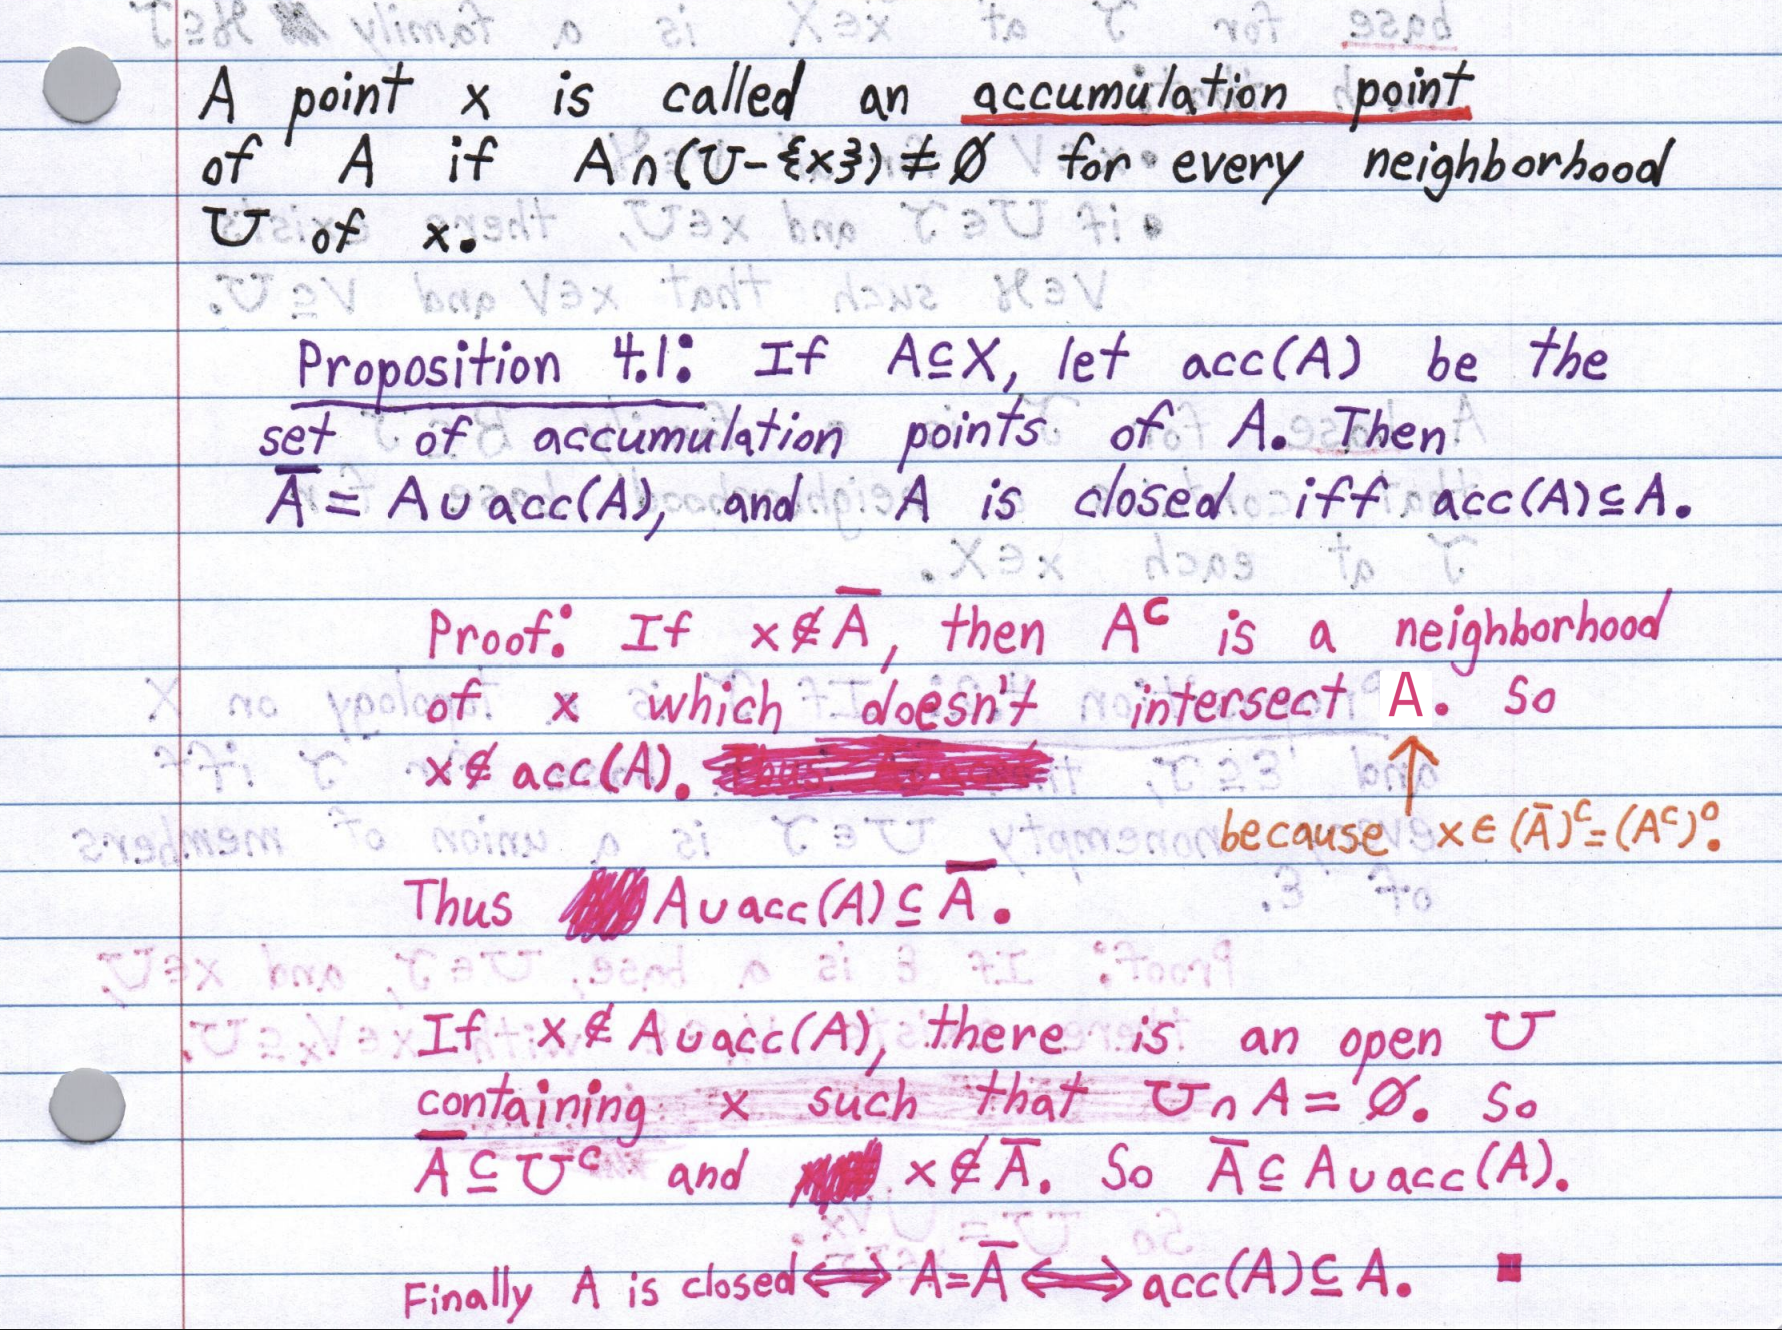
\includegraphics[scale=0.54]{HW2_1_math220a.png}\retTwo\par} & {\centering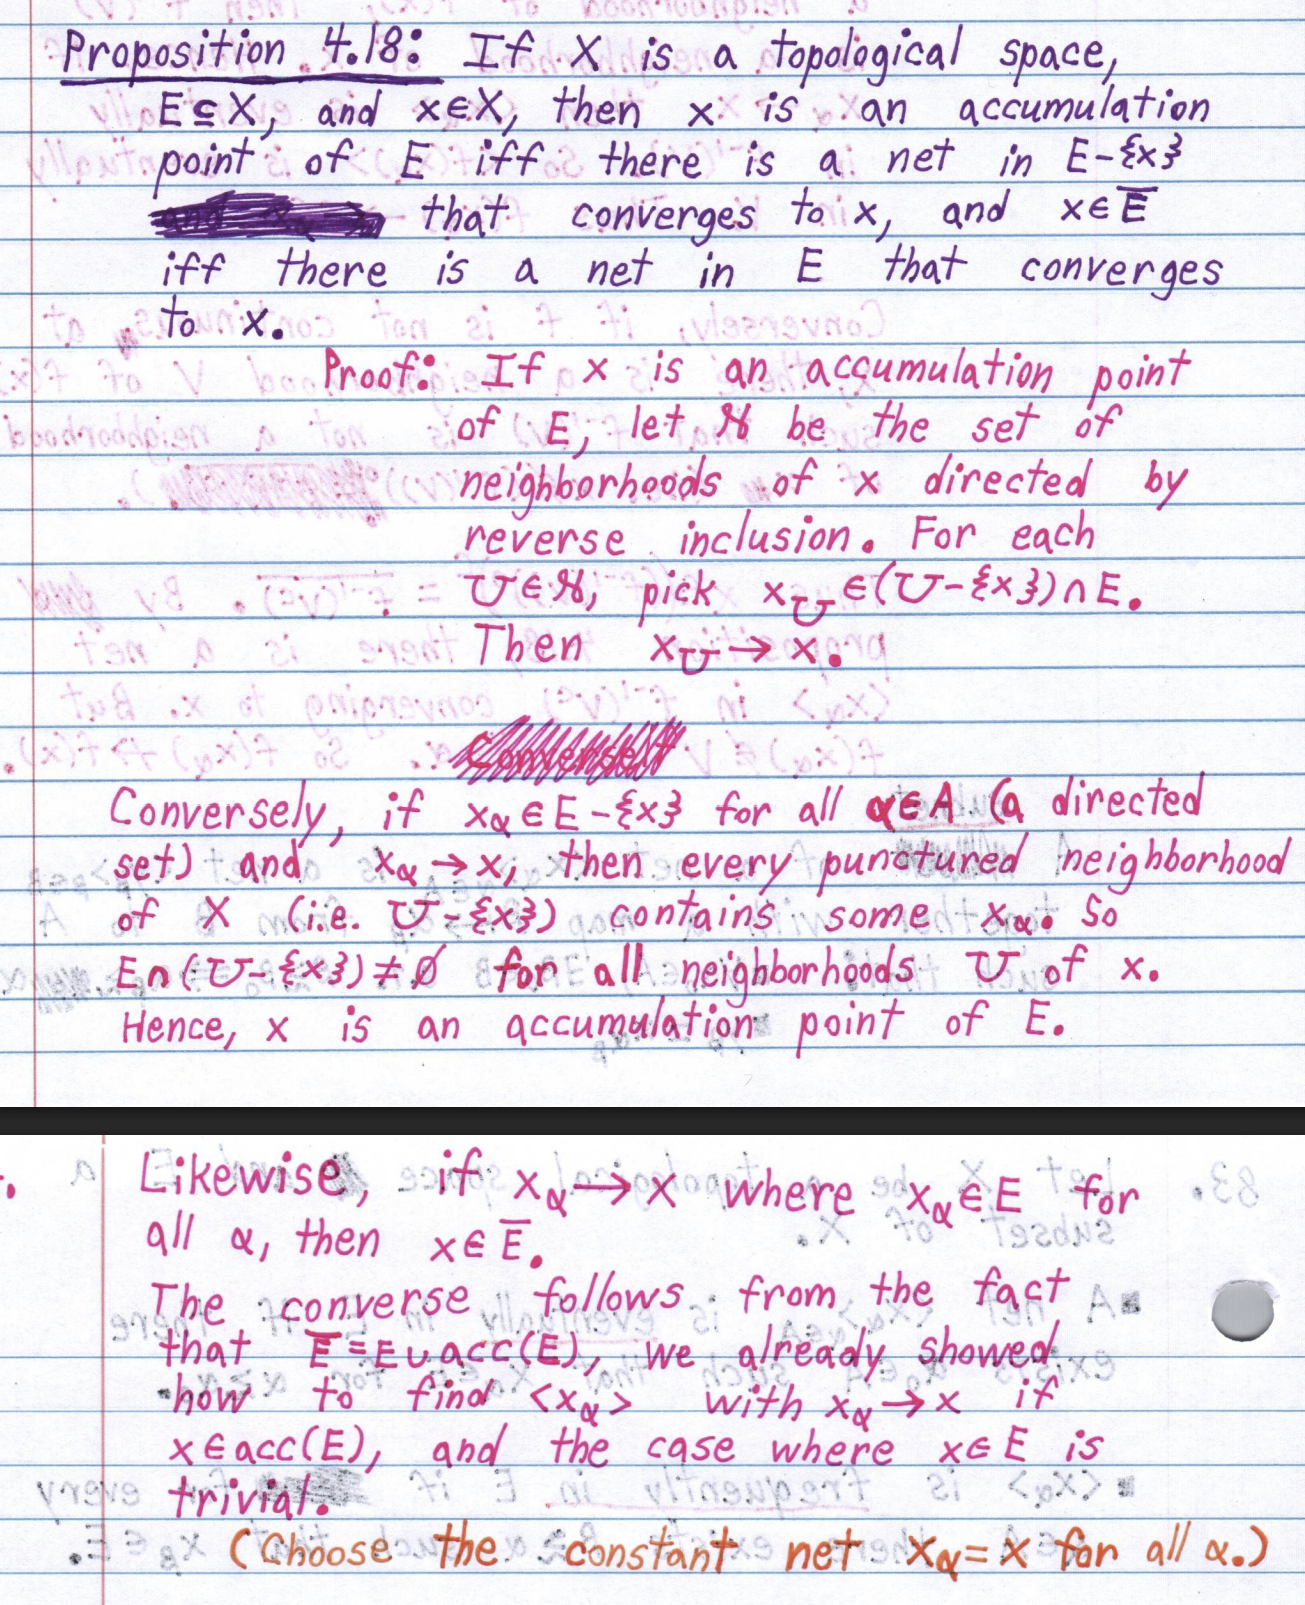
\includegraphics[scale=0.54]{HW2_2_math220a.png}\retTwo\par}
\end{tabular}\retTwo

\Hstatement\blab{Exercise II.3.4:} Let $z_n, z \in \mathbb{C}$ and let $d$ be the metric on $\mathbb{C}_\infty$. Then $|z_n - z| \to 0$ iff $d(z_n - z) \to 0$.

\begin{myIndent}\HexOne
	Recall that $d(z_n, z) = \frac{2|z_n - z|}{((|z_n|^2 + 1)(|z|^2 + 1))^{1/2}}$. Hence $d(x_n, z) \leq 2|z_n - z|$ and we have that $|z_n - z| \to 0 \Longrightarrow d(z_n - z) \to 0$.\retTwo
	
	On the other hand, if $\phi : \mathbb{C}_\infty \to S^2$ is the projection of the extended complex plane to\\ [1pt] the Riemann sphere, then by definition $d(z_n, z) \to 0$ iff $\phi(z_n) \to \phi(z)$ in $\mathbb{R}^3$. And since\\ [1pt] $\phi(z) \neq (0, 0, 1)$, there must exist some $-1 < C < 1$ and $N \in \mathbb{N}$ such that the third\\ [1pt] coordinates  of $\phi(z)$ and $\phi(z_n)$ are less than $C$ for all $n \geq N$. This translates to saying that:
	
	{\centering$\frac{|z|^2 - 1}{|z|^2 + 1}$ and $\frac{|z_n|^2 - 1}{|z_n|^2 + 1}$ are less than $C$ for all $n \geq N$.\retTwo\par}

	By quadratic formula this translate to saying that $|z_n|$ and $|z|$ are less than $D \coloneqq \frac{\sqrt{1 - C^2}}{1 - C}$\\ [-2pt] when $n \geq N$ So finally we may say that when $n \geq N$:

	{\center $|z_n - z| = \frac{1}{2}d(z_n, z)((|z_n|^2 + 1)(|z|^2 + 1))^{1/2} < \frac{1}{2}d(z_n, z)((D^2 + 1)(D^2 + 1))^{1/2}$ \retTwo\par}

	And now it's clear that $d(z_n - z) \to 0$ implies that $|z_n - z| \to 0$ as $n \to \infty$.\retTwo
\end{myIndent}

Also show that if $|z_n| \to \infty$, then $\{z_n\}_{n \in \mathbb{N}}$ is Cauchy in $\mathbb{C}_\infty$. 

\begin{myIndent}\HexOne
	To prove Cauchy-ness, it suffices to show $\{z_n\}_{n \in \mathbb{N}}$ converges to $\infty$. Fortunately, note that $d(z_n, \infty) - \frac{2}{(|z_n|^2 + 1)^{1/2}} \to 0$ as $|z_n| \to \infty$. So $z_n \to \infty$. $\blacksquare$\retTwo
\end{myIndent}

\blab{Exercise II.3.8:} Suppose $\{x_n\}_{n \in \mathbb{N}}$ is a Cauchy sequence in a metric space and $\{x_{n_k}\}_{k \in \mathbb{N}}$ is a convergent subsequence. Then $\{x_n\}$ is convergent.

\begin{myIndent}\HexOne
	Once again frick whoever is wasting all of our time with these stupid problems. Literally why I am wasting thousands of dollars to relearn content that any person getting into math grad school should already know.\retTwo

	Let $x$ be the limit of $\{x_{n_k}\}_{n \in \mathbb{N}}$ and pick any $\varepsilon > 0$.\newpage 
	
	Since $\{x_n\}_{n \in \mathbb{N}}$ is Cauchy there exists some $N \in \mathbb{N}$ such that $d(x_n, x_m) < \sfrac{\varepsilon}{2}$ for all\\ [1pt] $n, m \geq N$. Then because $x_{n_k} \to x$, we know there exists some $k \in \mathbb{N}$ such that\\ [1pt] $d(x_{n_k}, x) < \sfrac{\varepsilon}{2}$ and $n_k \geq N$. Thus, $d(x_n, x) \leq d(x_n, x_{n_k}) + d(x_{n_k}, x) < \varepsilon$ for all\\ [1pt] $n \geq N$. And this proves that $x_n \to x$ as $n \to \infty$. $\blacksquare$\retTwo
\end{myIndent}

\blab{Exercise II.4.1:} Prove that if every collection $\mathcalli{F}$ of closed subsets of $K$ with the finite intersection property has that $\bigcap_{F \in \mathcalli{F}} F \neq \emptyset$, then $K$ is compact.

\begin{myIndent}\HexOne
	Suppose $K$ is not compact and let $\{U_\alpha\}_{\alpha \in A}$ be an open cover of $K$ that has no finite\\ subcover. Then upon setting $F_\alpha = U_\alpha^\comp$ for all $\alpha \in A$ we have that $\{F_\alpha\}_{\alpha \in A}$ is a\\ collection of closed sets having the finite intersection property. After all, if there\\ were some $F_{\alpha_1}, \ldots, F_{\alpha_n}$ such that $\bigcap_{j=1}^n F_{\alpha_j} = \emptyset$ then that would imply that\\ [-1pt] $(\bigcap_{j=1}^n F_{\alpha_j})^\comp = \bigcup_{j=1}^n U_{\alpha_j} = K$. But that contradicts that $\{U_\alpha\}_{\alpha \in A}$ has no finite\\ [1pt] subcover of $K$.\retTwo

	At the same time though, $\bigcap_{\alpha \in A} F_\alpha = (\bigcup_{\alpha \in A} U_\alpha) = K^\comp = \emptyset$. So, we have found a\\ collection of closed sets with the finite intersection property whose intersection is\\ empty.  $\blacksquare$\retTwo
\end{myIndent}

\blab{Exercise II.4.4:} Show that the union of a finite number of compact sets is compact. 

\begin{myIndent}\HexOne
	Let $K_1, \ldots, K_n$ be a finite collection of compact sets and let $K$ be their union. Now if $\{U_\alpha\}_{\alpha \in A}$ is any open cover of $K$, then $\{U_\alpha\}_{\alpha \in A}$ is also an open cover of each $K_i$. So for each $i$ we can pick finitely many $U_{\alpha_j}$ covering each $K_i$. And by unioning the finitely many finite subcovers we get another finite subcover of all of $K$. $\blacksquare$\retTwo
\end{myIndent}

\blab{Exercise II.4.6:} Show that the closure of a totally bounded set is totally bounded.
\begin{myIndent}\HexOne
	Let $X$ be our metric space and suppose that $E \subseteq X$ is totally bounded. Then for any $\varepsilon > 0$ there are finitely many balls $B_1, \ldots, B_n$ of radius $\sfrac{\varepsilon}{2}$ covering $E$. And in turn the union of\\ [-1pt] the closures of those finitely many balls is a closed set containing $E$ and thus also $\overline{E}$. Finally, by expanding each of our balls to have radius $\varepsilon$ we now have a finite collection of balls of radius $\varepsilon$ covering $\overline{E}$.

	\begin{myIndent}\HexPPP
		Note to cover my bases:\\
		If $B_{\varepsilon/2}(x) \coloneqq \{y \in X : d(x, y) < \varepsilon/2\}$, then $\overline{B_{\varepsilon/2}(x)} \subseteq \{y \in X : d(x, y) \leq \varepsilon/2\}$ since the latter is easily checked to be closed set (it's complement is open by triangle inequality) which contains $B_{\varepsilon/2}(x)$. Also, $\{y \in X : d(x, y) \leq \varepsilon/2\} \subseteq \{y \in X : d(x, y) < \varepsilon\}$. $\blacksquare$\retTwo
	\end{myIndent}
\end{myIndent}

\blab{Exercise II.5.5:} Suppose $f: X \to \Omega$ is uniformly continuous (where $(\Omega, \rho)$ and $(X, d)$ are metric spaces). If $\{x_n\}_{n \in \mathbb{N}}$ is a Cauchy sequence in $X$ then $\{f(x_n)\}_{n \in \mathbb{N}}$ is a Cauchy sequence in $\Omega$.

\begin{myIndent}\HexOne
	Proof:\\
	For any $\varepsilon > 0$ pick $\delta > 0$ such that $\rho(f(x), f(y)) < \varepsilon$ whenever $d(x, y) < \varepsilon$. Since $\{x_n\}_{n \in \mathbb{N}}$ is a Cauchy sequence there exists some $N \in \mathbb{N}$ such that $d(x_n, x_m) < \delta$ for all $n, m \geq N$. And in turn $\rho(f(x_n), f(x_m)) < \varepsilon$ for all $n, m \geq N$. This proves that $\{f(x_n)\}_{n \in \mathbb{N}}$ is a Cauchy sequence in $\Omega$.\retTwo
\end{myIndent}

Does the prior statement still hold if $f$ is only assumed to be continuous but not\\ uniformly continuous.
\begin{myIndent}\HexOne
	No. For example, consider the sequence $\{\frac{1}{n}\}_{n \in \mathbb{N}}$ in $(0, \infty)$. This sequence is Cauchy since\\ for every $\varepsilon > 0$ we may choose some $N$ such that $\frac{1}{N} < \varepsilon$. And then for all $n, m \geq N$ we have that $|\frac{1}{n} - \frac{1}{m}| < \max(\frac{1}{n}, \frac{1}{m}) < \frac{1}{N} < \varepsilon$.\newpage

	Next let $f(x) = \frac{1}{x}$. To show that $f$ is continuous on $(0, \infty)$, note that both $1$ and $x$ are continuous on $(0, \infty)$. After all, just set $\delta = \varepsilon$ when doing the $\varepsilon$-$\delta$-proof. And since $x \neq 0$ on $(0, \infty)$, we have by proposition 5.5 in Conway that $\sfrac{1}{x}$ is continuous on $(0, \infty)$.\retTwo

	But now $\{\frac{1}{(1/n)}\}_{n \in \mathbb{N}}$ is not Cauchy. After all, for all $n,m \in \mathbb{N}$ with $n \neq m$ we have that:
	
	{\centering$|\frac{1}{(1/n)} - \frac{1}{(1/m)}| = |n - m| \geq 1$. $\blacksquare$\retTwo\par}
\end{myIndent}

\hTwo That's all my my math 220a homework for this week. Yay I'm done (finally). God I hope this class stops being a giant waste of money at some point. Anyways the next notes for this class will be on \inLinkRap{math 220a lecture 6}{page \_\_\_}.\retTwo

\mySepTwo

\hypertarget{Ergodic reading group notes 2}{My} next order of business for tonight is to continue taking notes for the reading group tomorrow. I'm picking up from \inLinkRap{Ergodic reading group notes 1 back}{here}.\retTwo

Let $(Y, T)$ be a dynamical system, $K$ be  a metrized compact group, and $\psi: Y \to K$ be a\\ continuous mapping. Then define $X = Y \times K$ and $T^\prime: X \to X$ by $T^\prime(y, k) = (Ty, \psi(y)k)$.\\ The resulting system is called a \udefine{group extension} or \udefine{skew product}  of $(Y, T)$ with $K$.

\begin{myIndent}\pracTwo
	Sanity check:
	\begin{enumerate}
		\item $T^\prime$ is a continuous map. After all, it's continuous iff its two output coordinates are individually continuous. And since we're already requiring $T$ and $\psi$ to be continuous and we know $(k_1, k_2) \mapsto k_1k_2$ is continuous from $K \times K$ to $K$, we can easily show both coordinates are continuous.\retTwo 
		
		\item If we define $\phi: X \to Y$ by $\phi(y, k) = y$, then $\phi$ is continuous (this is just a defining property of product topologies) and:
		
		{\centering$\phi(T^\prime(y, k)) = \phi(Ty, \psi(y)k) = Ty = T\phi(y, k)$.\retTwo\par}

		So, $\phi$ defines a homomorphism of $(X, T^\prime)$ to $(Y, T)$ and we've shown that $(X, T^\prime)$ does extend $(Y, T)$ by our prior definition.\retTwo
	\end{enumerate}
\end{myIndent}

\hTwo Note that in our above system, $X \curvearrowleft K$ by right translation. Specifically, for each $k^\prime \in K$ there exists a homeomorphism $R_{k^\prime} : X \to X$ given by $R_{k^\prime}(y, k) = (y, kk^\prime)$. Also, $R_k$ commutes with $T^\prime$ since:

{\centering $R_{k^\prime}(T^\prime(y, k)) = R_{k^\prime}(Ty, \phi(y)k) = (Ty, \phi(y)kk^\prime) = T^\prime(y, kk^\prime) = T^\prime(R_{k^\prime}(y, k))$ \retTwo\par}

Thus, each $R_{k^\prime}$ is an automorphism of the dynamical system $(X, T^\prime)$.


\begin{myIndent}\myComment 
	Side note:\\
	I think the author's choice to use right translations instead of left translations is really weird because it makes it so $R_{k_2}(R_{k_1}(y, k)) = (y, kk_1k_2) = R_{k_1k_2}(y, k)$. To fix this I would have instead set $T^\prime(y, k) = (Ty, k\psi(y))$ when defining the group extension, and then I'd have made $K \curvearrowright X$ by left translation. That way, we still have that $(X, T^\prime)$ is a dynamical system, $\phi$ is still a homomorphism from $(X, T^\prime)$ to $(Y, T)$, but now additionally we have that $R_{k_2} \circ R_{k_1} = R_{k_2k_1}$. Unfortunately, I don't want to confuse other presenters later on so I'll stick to the conventions of the book. :\lparen\newpage

	Also just to be clear: I shall denote $X \curvearrowleft G$ instead of $G \curvearrowright X$ when $G$ is acting from the right on $X$ instead of from the left.\retTwo
\end{myIndent}

\pracOne\mySepTwo
Before moving on to the next theorem, I need to clear up some confusion and write a few theorems.\retTwo

Firstly, recall on \hypertarget{Furstenberg confusion 1}{page 268} when I said a point $x$ is recurrent for $(X, T)$ if for any\\ neighborhood $V$ of $x$ there exists $n \geq 1$ with $T^n x \in V$. And then I said that that is\\ equivalent to saying that there is some increasing sequence $(n_k)_{k \in \mathbb{N}} \subseteq \mathbb{N}$ such that\\ $T^{n_k}x \to x$. Why are these two definitions equivalent?

\begin{myIndent}\pracTwo
	$(\Longleftarrow)$\\
	This direction is obvious.\retTwo

	$(\Longrightarrow)$\\
	If $T^n(x) = x$ for some $n$, then we know that $T^{kn}(x) = x$ for all $k \in \mathbb{N}$ and then we trivially have that $T^{kn}(x) \to x$ as $k \to \infty$. Meanwhile, suppose $T^n(x) \neq x$ for any $n \in \mathbb{N}$ and let $\{U_k\}_{k \in \mathbb{N}}$ be a countable decreasing neighborhood base for $x \in X$. Then we may construct a subsequence $\{T^{n_k}\}_{k \in \mathbb{N}}$ converging to $k$ as follows:
	\begin{myIndent}
		To start off, just pick any $n_1 \in \mathbb{N}$ such that $T^{n_1}x \in U_1$. Then we proceed by recursive definition.\retTwo
		
		Suppose we have already chosen $n_1 < \cdots < n_k$ in $\mathbb{N}$ and that $T^{n_i}x \in V_{i}$ for all\\ $1 \leq i \leq k$.  If $X$ is Hausdorff (which it will always be if $X$ is a metric space), then we can find pairs of disjoint open sets $V_{j}, W_j \subseteq X$ for all $1 \leq j \leq n_{k}$ such that $x \in V_j$ and $T^{j}x \in W_j$. And by setting $V \coloneqq \bigcap_{j=1}^{n_k} V_j$ we have that $V$ is an open set containing $x$ such that $T^j x \notin V$ for all $1 \leq j \leq n_k$.\retTwo

		Now pick $m \geq k + 1$ such that $U_m \subseteq V$. Then by assumption, there is some $n_{k+1} \in \mathbb{N}$ such that $T^{n_{k+1}} x \in U_m$. And also we must have that $n_{k+1} > n_k$. $\blacksquare$\retTwo
	\end{myIndent}
\end{myIndent}

More generally, given a dynamical system $(X, T)$ and any $x \in X$, define the \udefine{forward orbit closure} of $x$ as $Q(x) \coloneqq \overline{\{T^n x : n \geq 1\}}$. Note that $x$ is recurrent for $(X, T)$ iff $x \in Q(x)$.\\ [1pt] Also, by slightly modified reasoning to before, we know (even for $z \neq x$) that $z \in Q(x)$ iff\\ [1pt] there is some increasing sequence $\{n_k\}_{k \in \mathbb{N}}$ in $\mathbb{N}$ such that $T^{n_k} \to z$. \retTwo

\ul{Lemma A:} Let $(X, T)$ be a dynamical system and suppose that $y \in Q(x)$ and $z \in Q(y)$.\\ Then $z \in Q(x)$.
\begin{myIndent}\pracTwo
	Proof:\\
	Let $T^{n_j}y \to z$ as $j \to \infty$ and $T^{n_i}x \to y$ as $i \to \infty$. Also let $\{U_k\}_{k \in \mathbb{N}}$ be a countable decreasing neighborhood base for $z \in X$. We can construct a sequence $\{T^{n_k}x\}_{k \in \mathbb{N}}$ converging to $0$ as follows:
	\begin{myIndent}
		We'll want to keep track of subsequences of $\{n_{j(k)}\}_{k \in \mathbb{N}}$ and $\{n_{i(k)}\}_{n \in \mathbb{N}}$ of $\{n_j\}_{j \in \mathbb{N}}$ and $\{n_k\}_k \in \mathbb{N}$ respectively as we are constructing our actual desired sequence.\newpage

		For any $k$ pick $j(k) \in \mathbb{N}$ such that $T^{n_{j(k)}}y \in U_k$ and $j(k) > j(k-1)$ (if $k > 1)$. Then set $V = (T^{n_j})^{-1}(U_k)$. Because $V$ is an open neighborhood of $y$, we know that there is some $I \in \mathbb{N}$ such that $T^{n_i}x  \in V$ whenever $i \geq I$. So pick $i(k)$ such that $T^{n_{i(k)}}x \in V$ and $i(k) > i(k-1)$ (if $k > 1$). Now $T^{n_{j(k)} + n_{i(k)}} x \in U_k$.\retTwo

		Doing this for all $K \in \mathbb{N}$, we get that $T^{n_{j(k)} + n_{i(k)}} x \to z$ as $k \to \infty$ and that\\ $\{n_{j(k)} + n_{i(k)}\}_{k \in \mathbb{N}}$ is increasing. $\blacksquare$\retTwo
	\end{myIndent}
\end{myIndent}

\ul{Lemma B:} Suppose $(X, T)$ is a dynamical system and $R$ is an automorphism of $(X, T)$\\ (meaning $R \circ T = T \circ R$ and $R : X \to X$ is continuous). Then for any $x \in X$ we have\\ that $R(Q(x)) \subseteq Q(Rx)$.

\begin{myIndent}\pracTwo
	Proof:\\
	Suppose $z \in Q(x)$ and let $T^{n_k}x \to z$ Then $R(z) = \lim_{k \to \infty} R(T^{n_k}x) = \lim_{k \to \infty}T^{n_k}(Rx)$. So $R(z) \in Q(Rx)$ and we've shown that $R(Q(x)) \subseteq Q(Rx)$.\retTwo
\end{myIndent}

\ul{Lemma C:} Suppose $K$ is a compact metrized group and $k \in K$. Then the sequence $\{k^n\}_{n \in \mathbb{N}}$ has the identity $e$ of $K$ as a subsequential limit.

\begin{myIndent}\pracTwo
	Proof:\\
	We know that $k^n$ must have a subsequential limit since it's a sequence in a compact set. So call this limit $g$ and say that $k^{n_j} \to g$ as $j \to \infty$. Since inversion is continuous on $K$, we thus know that $k^{-n_j} \to g^{-1}$ as $j \to \infty$. Also, since the group product is continuous on $K$, we know that $k^{n_{2j}}k^{-n_j} = k^{n_{2j} - n_j} \to gg^{-1} = e$ as $j \to \infty$. Finally, note that $n_{2j} - n_j \geq j$ for all $j$. And so there must be some subsequence $\{j_{k}\}_{k \in \mathbb{N}}$ such that $n_{2j_k} - n_{j_k}$ is strictly increasing. $\blacksquare$\retTwo
\end{myIndent}

I think before next week I will try to read up on topological groups some more cause I feel like I have a knowledge gap right now.\\
\mySepTwo

\exTwo\ul{Theorem 1.4:} If $y_0 \in Y$ is recurrent for $(Y, T)$ and $(X, T^\prime)$ is a skew extension of $(Y, T)$, then $(y_0, k_0)$ is a recurrent point of $(X, T^\prime)$ for all $k_0 \in K$.
\begin{myIndent}\exThreeP
	Proof:\\
	Let $e$ denote the identity of $K$. We shall show $(y_0, e)$ is a recurrent point of $(X, T)$ since it then follows from \inLinkRap{Furstenberg proposition 1.3}{proposition 1.3:} that each $R_{k_0}(y_0, e) = (y_0, k_0)$ is recurrent.\retTwo

	For any $x \in X$ let $Q(x) = \overline{\{(T^\prime)^n x : n \geq 1\}}$ denote the \udefine{forward orbit closure} of $x$. Then $x$ is recurrent for $(X, T^\prime)$ iff $x \in Q(x)$. Now since $y_0$ is recurrent for $(Y, T)$, there is some $k_1 \in K$ such that: $(y_0, k_1) \in Q(y_0, e)$.

	\begin{myIndent}\exPPP
		Why (since Furstenberg doesn't explain this)?\\ [4pt]
		Note that $(T^\prime)^n(y_0, e) = (T^n y_0, k^{(n)})$ where:
		
		{\centering$k^{(n)} = \phi(T^{n-1} y_0 ) \phi( T^{n-2} y_0) \cdots \phi(T y_0)\phi(y_0)$.\retTwo\par}

		Now because $y_0$ is recurrent for $(Y, T)$, we know that there is a subsequence\\ $\{T^{n_i} y\}_{i \in \mathbb{N}}$ such that $T^{n_i} y \to y$ as $i \to \infty$. And since $K$ is compact, we have that $\{k^{n_{i}}\}_{i \in \mathbb{N}}$ has a subsequential limit point $k_1$. And finally, by passing to another subsequence $\{n_{i_j}\}_{j \in \mathbb{N}}$ we get that $(T^\prime)^{n_{i_j}}(y_0, e) \to (y_0, k_1)$ as $j \to \infty$.\newpage
	\end{myIndent}

	But now note by induction that $(y_0, k_1^n) \in Q(y_0, e)$ for all $n \in \mathbb{N}$.

	\begin{myIndent}\exPPP
		Why?\\
		We know $(y_0, k_1) \in Q(y_0, e)$. Now by induction assume that $(y_0, k_1^n) \in Q(y_0, e)$. Then $(y_0, k_1^{n+1}) = R_{k_1}(y_0, k_1^n)  \in Q(R(y_0, e)) = Q(y_0, k_1)$ by lemma B. But we also have that $(y_0, k_1) \in Q(y_0, e)$. So $(y_0, k_1^{n+1}) \in Q(y_0, e)$ by lemma A.\retTwo
	\end{myIndent}

	In turn by lemma C we have that there is an increasing subsequence $\{n_j\}_{j \in \mathbb{N}}$ such that $(y_0, k^{n_j}) \to (y_0, e)$ as $j \to \infty$. And since $Q(y_0, e)$ is closed, we thus have shown that $(y_0, e) \in Q(y_0, e)$. $\blacksquare$\retTwo
\end{myIndent}

\hTwo By using the prior theorems we can inductively obtain examples of non-Kronecker\\ dynamical systems where every point is recurrent.\retTwo

For example, let $T : \mathbb{T}^2 \to \mathbb{T}^2$ be given by $T(\theta, \phi) = (\theta + a, \phi + 2\theta + a)$. Then $(\mathbb{T}^2, T)$ is a group extension of the Kronecker system $(\mathbb{T}, T^\prime)$ where $T^\prime \theta = \theta + a$ and $\psi(\theta) = 2\theta + a$. By theorems 1.2. and 1.4 we know that every point in $(\mathbb{T}^2, T)$ is recurrent.

In the prior system note that the orbit of $(0, 0) \in \mathbb{T}^2$ is:

{\centering\begin{tabular}{l}
	$(0, 0) \to (a, a) \to (2a, 4a) \to \cdots \to (na, n^2 a)$\\ [4pt]
	$\phantom{(0, 0) \to (a, a) \to (2a, 4a) \to \cdots} \to (na + a, n^2a + 2na + a) = ((n+1)a, (n^2 +2n + 1)a)$\\ [4pt]
	$\phantom{(0, 0) \to (a, a) \to (2a, 4a) \to \cdots \to (na + a, n^2a + 2na + a)} = ((n+1)a, (n+1)^2a) \to \cdots$ 
\end{tabular}\retTwo\par}

This leads to the following proposition:

\begin{myIndent}\exTwo
	\ul{Proposition 1.5:} For any $\alpha \in \mathbb{R}$ and $\varepsilon > 0$ we can solve the diophantine inequality $|\alpha n^2 - m| < \varepsilon$ (where $n > 0$).

	\begin{myIndent}\exThreeP
		Proof:\\
		We know there is some increasing sequence $\{n_k\}_{k \in \mathbb{N}}$ in $\mathbb{N}$ such that\\ $(n_k a, n_k^2 a) \to (0, 0) \in \mathbb{T}^2$. In particular, since $n_k^2 a \to 0 \in \mathbb{T}$ we know that\\ if $k$ is fixed large enough, then there exists $m \in \mathbb{N}$ such that $|n_k^2 - m| < \varepsilon$. $\blacksquare$\retTwo
	\end{myIndent}
\end{myIndent}

We can extend this to higher degree polynomials too. Let $p(x)$ be a polynomial of degree $d$ with real coefficients and write $p_d(x) \coloneqq p(x)$ as well as:

{\centering $p_{d-1}(x) \coloneqq p_d(x + 1) - p_d(x)$, $\phantom{a}p_{d-2}(x) \coloneqq p_{d-1}(x + 1) - p_{d-1}(x)$, etc. \retTwo\par}

Each $p_i(x)$ is of degree $i$. Let $\alpha$ be the constant $p_0(x)$. Then define a transformation\\ $T: \mathbb{T}^d \to \mathbb{T}^d$ by $T(\theta_1, \theta_2, \theta_3 \ldots, \theta_d) \coloneqq (\theta_1 + \alpha, \theta_2 + \theta_1, \theta_3 + \theta_2, \ldots, \theta_d - \theta_{d-1})$.

\begin{myIndent}\pracTwo
	By induction, we can see that this is a group extension of a dynamical system on the $(d-1)$-torus which in turn is a group extension of a dynamical system on the $(d-2)$-torus, and so on and so forth down to the $1$-torus. So we can conclude that each point in $\mathbb{T}^d$ is recurrent.\retTwo

	\exThreeP I'll do a step of the induction cause why not.
	\begin{myIndent}\exPPP
		Suppose we've shown that $(\mathbb{T}^{k}, T_k)$ is a dynamical system where:
		
		{\centering$T_k(\theta_1, \theta_2, \ldots, \theta_k) = (\theta_1 + \alpha, \theta_2 + \theta_1, \theta_3 + \theta_2, \ldots, \theta_k - \theta_{k-1})$.\retTwo\par}

		Then by letting $\psi : \mathbb{T}^k \to \mathbb{T}$ be given by $\psi(\theta_1, \theta_2, \ldots, \theta_k) = \theta_k$ we have that $(\mathbb{T}^k, T_{k+1})$ is a group extension where:

		{\centering\begin{tabular}{l}
			$T_{k+1}(\theta_1, \ldots, \theta_{k+1}) = (T_k(\theta_1, \dots, \theta_{k}), \theta_{k+1} + \psi(\theta_1, \dots, \theta_{k}))$\\ [4pt]
			$\phantom{T_{k+1}(\theta_1, \ldots, \theta_{k+1})} = ((\theta_1 + \alpha, \theta_2 + \theta_1, \ldots, \theta_{k} + \theta_{k-1}), \theta_{k+1} + \theta_k)$.
		\end{tabular} \newpage\par}
	\end{myIndent}
\end{myIndent}

Now compute the orbit of $(p_1(0), \ldots, p_d(0))$. Since $p_{i-1}(n) + p_i(n) = p_i(n + 1)$ we find that $T(p_1(n), p_2(n), \ldots, p_d(n)) = (p_1(n + 1), p_2(n+1), \ldots, p_d(n+1))$.\retTwo

And thus $T^n(p_1(0), p_2(0), \ldots, p_d(0)) = (p_1(n), p_2(n), \ldots, p_d(n))$.\retTwo

We conclude that $p_d(n) = p(n)$ must get arbitrarily close to $p(0)$ modulo $1$. Hence the following theorem:
\begin{myIndent}
\exTwo\ul{Theorem 1.6:} If $p(x)$ is any real polynomial with $p(0) = 0$, then for any $\varepsilon > 0$ we can solve the diophantine inequality $|p(n) - m| < \varepsilon$ (where $n > 0$).\retTwo
\end{myIndent}

I'll study more related to this reading group on \inLinkRap{Ergodic reading group notes 3}{page \_\_\_}.

\mySepTwo

\dispDate{10/8/2025}

\blect{Math 200a Homework:}\retTwo

\Hstatement\blab{Set 2 Problem 1:} Suppose $G$ is a simple group (meaning the only normal subgroups of $G$ are $\{1\}$ and $G$), and it has a subgroup $H$ of index $n$ where $n$ is an integer more than $1$. Prove that $G$ can be embedded into the symmetric group $S_n$.
\begin{myIndent}\HexOne
	Consider the action $G \curvearrowright G/H$ by left translation, and let $\phi: G \to S_{G/H}$ be the group homomorphism induced by this action. Note that since $[G : H] = n$, we know $S_{G/H} \cong S_n$.\\ [1pt] So, as long as we can prove that $\phi$ is injective then we will be done.\retTwo

	Suppose $x \in \ker(\phi)$. Then we know that $xgH = gH$ for all $g \in G$. But that's true iff\\ $x \in gHg^{-1}$ for all $g \in G$. Or in other words, we must have that $x \in \core_G(H)$. This\\ proves that $\{1\} < \ker(\phi) < \core_G(H)$. Next note that because $H \neq G$ (which we\\ know since $n > 1$), $\core_G(H) \lhd G$, $\core_G(H) < H$, and $G$ is simple, we must have that\\ $\core_G(H) = \{1\}$. So, we've shown that $\ker(\phi) = \{1\}$. And this proves that $\phi$ is injective.\\ $\blacksquare$\retTwo
\end{myIndent}

\blab{Set 2 Problem 7:} Suppose $N$ is a finite cyclic normal subgroup of $G$. Prove that every subgroup of $N$ is normal in $G$.
\begin{myIndent}\HexOne
	
\end{myIndent}






% ~~~~~~~~~~~~~~~~~~~~~~~~~~~~~~~~~~~~~~~~~~~~~~

\hypertarget{bib citation 12}{}
\hypertarget{Ergodic reading group notes 3}{}
\hypertarget{Ergodic reading group notes 1 back}{}
\hypertarget{Furstenberg proposition 1.3}{}


\hypertarget{math 241a lecture 3}{}
\hypertarget{math 200a lecture 6}{}
\hypertarget{math 220a lecture 6}{}
\hypertarget{bib citation 13}{}
\hypertarget{page idk 1 reference}{}
\hypertarget{Folland Proposition 10.1}{}
\hypertarget{Alireza lemma page 256}{}



\end{document}




